% =============================================================================
% COPYRIGHT AND DISCLAIMER
% =============================================================================
% This file is provided as a convenience template for competition participants.
% By using it, you accept full responsibility for compliance with all applicable
% copyright, licensing, and usage rules of the Association for Computing
% Machinery (ACM) and of any LaTeX packages you load (including, without
% limitation, the "acmart" document class and related ACM materials).
%
% Consult ACM's official publication, template, and copyright policies before
% using this setup for any purpose other than this competition. Do not assume
% that this template may be reused, redistributed, or submitted elsewhere
% without independently verifying ACM's current rules.
%
% Use of the "acmart" class, the "sigconf" option, or ACM-style formatting in
% this template does NOT mean that this report, this competition, its organizers,
% or any resulting PDF is sponsored, endorsed, affiliated with, or published by
% ACM. ACM trademarks and branding remain the property of ACM.
%
% Template packages live in preamble.tex.
% Citations live in main.bib. Edit this file with your paper content.
% =============================================================================

\documentclass[sigconf]{acmart}
\usepackage{placeins} % Keep floats within their respective subsections
% =============================================================================
% Template setup — participants normally do not edit this file.
% Author content belongs in main.tex; citations belong in main.bib.
% \documentclass lives in main.tex so Overleaf does not treat this file as root.
% =============================================================================

% --- Competition / non-ACM-submission friendly rights metadata -------------
\setcopyright{none}
\settopmatter{printacmref=false}
\acmConference[Kaggle Competition]{Filament Segmentation Challenge}{2026}{\href{https://www.kaggle.com/competitions/filament-segmentation-2026}{kaggle.com/competitions/filament-segmentation-2026}}
\acmBooktitle{Competition Report}
\acmDOI{}
\acmISBN{}

% --- Author guidance text --------------------------------------------------
% \guide{...} is gray italic while \guideStyletrue; omitted from the PDF if false.
% Flip the switch in main.tex after % =============================================================================
% Template setup — participants normally do not edit this file.
% Author content belongs in main.tex; citations belong in main.bib.
% \documentclass lives in main.tex so Overleaf does not treat this file as root.
% =============================================================================

% --- Competition / non-ACM-submission friendly rights metadata -------------
\setcopyright{none}
\settopmatter{printacmref=false}
\acmConference[Kaggle Competition]{Filament Segmentation Challenge}{2026}{\href{https://www.kaggle.com/competitions/filament-segmentation-2026}{kaggle.com/competitions/filament-segmentation-2026}}
\acmBooktitle{Competition Report}
\acmDOI{}
\acmISBN{}

% --- Author guidance text --------------------------------------------------
% \guide{...} is gray italic while \guideStyletrue; omitted from the PDF if false.
% Flip the switch in main.tex after % =============================================================================
% Template setup — participants normally do not edit this file.
% Author content belongs in main.tex; citations belong in main.bib.
% \documentclass lives in main.tex so Overleaf does not treat this file as root.
% =============================================================================

% --- Competition / non-ACM-submission friendly rights metadata -------------
\setcopyright{none}
\settopmatter{printacmref=false}
\acmConference[Kaggle Competition]{Filament Segmentation Challenge}{2026}{\href{https://www.kaggle.com/competitions/filament-segmentation-2026}{kaggle.com/competitions/filament-segmentation-2026}}
\acmBooktitle{Competition Report}
\acmDOI{}
\acmISBN{}

% --- Author guidance text --------------------------------------------------
% \guide{...} is gray italic while \guideStyletrue; omitted from the PDF if false.
% Flip the switch in main.tex after \input{preamble}.
%
% Do not use \guide{...} for \email{...}.
\usepackage{xcolor}
\newif\ifguideStyle
\guideStyletrue
\newcommand{\guide}[1]{%
  \ifguideStyle
    {\color{gray!65}\itshape #1}%
  \fi
}

% --- Math ------------------------------------------------------------------
% Do NOT load amssymb (or amsfonts): acmart already loads newtxmath, which
% defines the same symbols (e.g. \Bbbk) and causes a conflict on Overleaf.
% amsmath is already provided by acmart; mathtools extends it.
\usepackage{mathtools}

% --- Figures ---------------------------------------------------------------
% graphicx is already loaded by acmart
\usepackage{subcaption}

% --- Tables ----------------------------------------------------------------
% booktabs is already loaded by acmart
\usepackage{tabularx}
\usepackage{multirow}

% --- Bibliography style is set in main.tex (ACM-Reference-Format) ----------
.
%
% Do not use \guide{...} for \email{...}.
\usepackage{xcolor}
\newif\ifguideStyle
\guideStyletrue
\newcommand{\guide}[1]{%
  \ifguideStyle
    {\color{gray!65}\itshape #1}%
  \fi
}

% --- Math ------------------------------------------------------------------
% Do NOT load amssymb (or amsfonts): acmart already loads newtxmath, which
% defines the same symbols (e.g. \Bbbk) and causes a conflict on Overleaf.
% amsmath is already provided by acmart; mathtools extends it.
\usepackage{mathtools}

% --- Figures ---------------------------------------------------------------
% graphicx is already loaded by acmart
\usepackage{subcaption}

% --- Tables ----------------------------------------------------------------
% booktabs is already loaded by acmart
\usepackage{tabularx}
\usepackage{multirow}

% --- Bibliography style is set in main.tex (ACM-Reference-Format) ----------
.
%
% Do not use \guide{...} for \email{...}.
\usepackage{xcolor}
\newif\ifguideStyle
\guideStyletrue
\newcommand{\guide}[1]{%
  \ifguideStyle
    {\color{gray!65}\itshape #1}%
  \fi
}

% --- Math ------------------------------------------------------------------
% Do NOT load amssymb (or amsfonts): acmart already loads newtxmath, which
% defines the same symbols (e.g. \Bbbk) and causes a conflict on Overleaf.
% amsmath is already provided by acmart; mathtools extends it.
\usepackage{mathtools}

% --- Figures ---------------------------------------------------------------
% graphicx is already loaded by acmart
\usepackage{subcaption}

% --- Tables ----------------------------------------------------------------
% booktabs is already loaded by acmart
\usepackage{tabularx}
\usepackage{multirow}

% --- Bibliography style is set in main.tex (ACM-Reference-Format) ----------


% Guide styling: \guideStyletrue = show gray italic hints; \guideStylefalse = omit them
% \guideStyletrue
\guideStylefalse

% Red marker for numbers / items that still need to be filled in (remove before submission)
\newcommand{\tbd}[1]{{\color{red}#1}}
% Placeholder box for figures (replace by \includegraphics when the figure is ready)
\newcommand{\figbox}[2]{\fbox{\parbox[c][#1][c]{0.94\linewidth}{\centering\color{gray}#2}}}

\begin{document}

\title{CompassNet: Orientation-Aware Network for Solar Filament Segmentation}

\subtitle{A Solution to the Solar Filament Segmentation Challenge 2026}

\author{José Alexandre Soares de Oliveira}

\affiliation{%
    \institution{Universidade de São Paulo}
    \city{São Paulo}
    \country{Brazil}
}

\email{josesoaresoliveira@usp.br}

\begin{abstract}
    This report describes our solution to the Solar Filament Segmentation Challenge~2026, a Kaggle competition on automatic segmentation of solar filaments in GONG H-$\alpha$ observations. 

    We propose CompassNet, a U-Net variant that couples a fixed Kirsch operator with a multi-head attention mechanism, so that filament geometry guides the separation of solar filaments from the background.

    We are motivated by the intuition that morphology is the most discriminative feature for solar filament segmentation. It is our understanding that other image features, such as pixel intensity, are not specific to filaments, since other structures on the disk, like clouds, shadows and sunspots, exhibit these features as well. CompassNet builds on the premise that attending to the orientation, position, and overall shape of solar structures improves segmentation in difficult tasks, such as segmenting barbs or preserving the continuity of long structures.

    To further improve our design, we also pretrain the network with masked image completion on roughly $5{,}000$ GONG images outside of the period covered by the challenge dataset.
\end{abstract}

\maketitle

% ==================================== %
%              INTRODUCTION            %
% ==================================== %
\section{Introduction}
    This report goes over the details of our submitted solution to the Solar Filament Segmentation Challenge~2026 \cite{filament-segmentation-2026}. The challenge, launched on July~10,~2026, is organized by the Earth-Space AI Research (ESAIR) Lab\footnote{\href{https://www.esairlab.com/home}{www.esairlab.com/}}. This challenge utilizes the MAGFiLO dataset for evaluation of the segmentation algorithms \cite{ahmadzadeh2024dataset}. 

    Segmenting solar filaments in H-$\alpha$ images poses various difficulties. First, one cannot rely on pixel intensity alone, as other magnetic solar structures, such as sunspots, have a similar intensity distribution \cite{ahmadzadeh2019filament_arxiv, solomon2025edgeattnet}. Moreover, the granular background texture of H-$\alpha$ images makes it difficult, and at times impossible even for human experts, to tell the fine-scale structures of a filament, namely its barbs, from the surrounding background \cite{ahmadzadeh2019filament_arxiv}. Finally, convolutional networks, a common choice for segmentation, rely on local receptive fields. This limits their ability to capture global context, which is important for segmenting solar filaments, as these are often long and thin \cite{solomon2025edgeattnet}.
    
    We believe that learning the typical morphology of filaments helps the model preserve structural continuity and capture barbs. In particular, it should avoid isolated islands, disconnected regions of the same filament, and implausible segments. To this end, we use a multihead-attention mechanism guided by a multiscale orientation field, as a way of forcing the model to capture geometric features of the image as its main learning signal. The source code is publicly available at \url{https://github.com/hermengardo/CompassNet_SolarFilamentChallenge_Solution}.

% ==================================== %
%              METHODOLOGY             %
% ==================================== %
\section{Methodology}\label{sec:methodology}

\subsection{Data Splitting}\label{sec:splitting}
The training data are the MAGFiLO annotations distributed with the challenge (COCO format). Each image has one or more annotators, and each annotator provides a set of filament polygons. The training annotations contain approximately 8,200 filament polygons (7,500 in the training split and 699 in the validation split) over roughly 650 training and 55 validation images.

To ensure representative coverage across solar cycles, we used the daily sunspot number from SILSO~\cite{silso}, calculated its monthly mean, and divided the months into three categories corresponding to low, moderate, and high activity. We then grouped the images into blocks of 90 days, labeled each block with its most frequent phase, and assigned each block entirely to either the training or the validation set.

The resulting phase distributions, expressed as fractions of the annotations in each split, are shown in Table~\ref{tab:phase}.

\begin{table}[!htbp]
    \centering
    \caption{Distribution of solar-cycle phases in the training and validation splits.}
    \label{tab:phase}
    \small
    \begin{tabular}{lcc}
        \toprule
        \textbf{Phase} & \textbf{Train} & \textbf{Validation} \\
        \midrule
        High     & 58.8\% & 54.9\% \\
        Moderate & 34.3\% & 34.3\% \\
        Low      & 6.9\%  & 10.7\% \\
        \bottomrule
    \end{tabular}
\end{table}
\FloatBarrier

To avoid temporal persistence of filaments leaking across the split boundary, we discarded from the training set every image captured less than 2 days from any validation image. We kept the minimum gap between train and validation low because we do not believe that the leakage is significant, and we wanted to avoid discarding too many images as the dataset is already small. For the final split (seed 567), 98.5\% of the remaining training images lie at least 7 days from the nearest validation image, and 57.1\% at least 90 days.

\subsection{Preprocessing}\label{sec:preprocessing}

We mostly adopted the preprocessing pipeline proposed by Solomon \textit{et al}.~\cite{solomon2025edgeattnet}. Each image is first scaled to the range \([0,1]\) and then processed through four successive steps: solar disk detection, radial flattening, CLAHE, and off-disk zeroing. Table~\ref{tab:preprocessing} lists the parameters of each step.

\begin{table}[H]
    \centering
    \caption{Preprocessing operations and their corresponding parameters.}
    \label{tab:preprocessing}
    \footnotesize
    \renewcommand{\arraystretch}{1.12}
    \setlength{\tabcolsep}{4pt}
    \begin{tabular}{@{}lll@{}}
        \toprule
        \textbf{Step} & \textbf{Parameter} & \textbf{Value} \\
        \midrule
        Disk detection & Working resolution & $256 \times 256$ \\
                       & Gaussian kernel    & $9 \times 9$, $\sigma=2$ \\
                       & Canny thresholds   & 30, 100 \\
                       & Contour filter     & area $\geq 1000$, $r > 40$, offset $< 50$ \\
                       & Fallback           & $r = 0.45 \cdot \min(\text{Height},\text{Width})$ \\
        \midrule
        Radial     & Ring width            & 1 pixel \\
        flattening & Smoothing window      & 21 samples \\
                   & Minimum profile value & 0.05 \\
        \midrule
        CLAHE & Tile grid     & $8 \times 8$ \\
              & Clip limit    & 2.0 \\
        \midrule
        Off-disk zeroing & -- & -- \\
        \bottomrule
    \end{tabular}
\end{table}

\subsection{Network Architecture}\label{sec:architecture}
CompassNet is a U-Net-style network built with a ResNet-34 \cite{he2016deep} encoder backbone and a decoder path of convolutional blocks. It uses an orientation field, computed at multiple scales from the input image, as an explicit directional prior, guiding an attention mechanism applied before the bottleneck, conditioning the intermediate decoder stages, and providing additional guidance to the full-resolution decoder block. Besides the usual encoder, decoder and skip connections that characterize a U-Net~\cite{ronneberger2015unetconvolutionalnetworksbiomedical, solomon2025edgeattnet}, CompassNet is composed of four other components:

\begin{itemize}
    \item \textbf{Kirsch Filters:} non-learnable filters initialized with the Kirsch operator.
    \item \textbf{Orientation Field Extractor:} reduces the Kirsch responses at each scale to a magnitude and two direction components.
    \item \textbf{Compass Attention:} applies windowed self-attention guided by the orientation field.
    \item \textbf{Orientation Conditioning:} uses the orientation field to condition intermediate decoder features at multiple resolutions.
\end{itemize}

\subsubsection{Kirsch Filters}\mbox{}\ 

To encode edge direction into the architecture, we use a non-learnable bank of $3 \times 3$ kernels initialized as the Kirsch compass operator. The Kirsch operator is an edge detector that responds to eight directions: N, NE, E, SE, S, SW, W, and NW. These eight orientation matrices are used to add information about local edge orientation to the network. 

To capture structure at multiple scales without losing local detail, we apply the kernels at $D$ different dilation rates. All dilations share the same set of eight kernels, ordered clockwise from north to northwest. 

The kernels are initialized with the Kirsch coefficients scaled by $1/15$, and sum to zero so that flat regions produce no response. The input image is standardized to zero mean and unit variance (per image) before filtering, and borders are handled with replicate padding, preserving the spatial size.

Each response is split, through a ReLU, into two channels: positive, which keeps the positive responses (positive weights indicate the side that is brighter than the opposite side), and a negative one, which keeps the negative responses with their sign flipped (the side that is darker). So, for an input image $I \in \mathbb{R}^{1 \times H \times W}$, the responses of all dilations are concatenated into a $16D$-channel tensor $\mathbf{R} \in \mathbb{R}^{16D \times H \times W}$.

\subsubsection{Orientation Field Extractor}\mbox{}\

For each scale, the positive and negative responses of each kernel are added together to obtain the absolute response, making the representation independent of contrast polarity. This prevents transitions from bright to dark and from dark to bright from being treated differently by the network. The resulting responses ($w_k$), are then summed across the eight directions to obtain the total edge response. Finally, we apply a logarithmic transformation to reduce the influence of large responses and obtain the edge magnitude at that scale ($m$):

\begin{equation}
m = \log\left(1 + \sum_{k=0}^{7} w_k\right).
\end{equation}

We also derive a direction vector from the responses by converting the eight filter directions into Cartesian coordinates. Since edge orientation is defined modulo $\pi$, we double the angles so that opposite directions produce the same vector rather than cancelling each other out. We then divide each component by the sum of the eight responses:

\begin{equation}
v_x = \frac{\sum_{k=0}^{7} w_k \cos 2a_k}{\sum_{k=0}^{7} w_k + \tau}, \qquad
v_y = \frac{\sum_{k=0}^{7} w_k \sin 2a_k}{\sum_{k=0}^{7} w_k + \tau},
\end{equation}

where $a_k = k\pi/4$ is the direction of the $k$-th kernel. Finally, adding a small constant $\tau$ to the denominator avoids division by zero and reduces the vector magnitude in regions with weak edge responses, since the smaller the sum of the responses is, the greater the influence of $\tau$ on the denominator, pulling both vector components closer to zero.

The expected effect is a vector field whose vectors respond strongly and coherently along edges. Figure~\ref{fig:vector_field} illustrates this effect.


\begin{figure}[H]
    \centering
    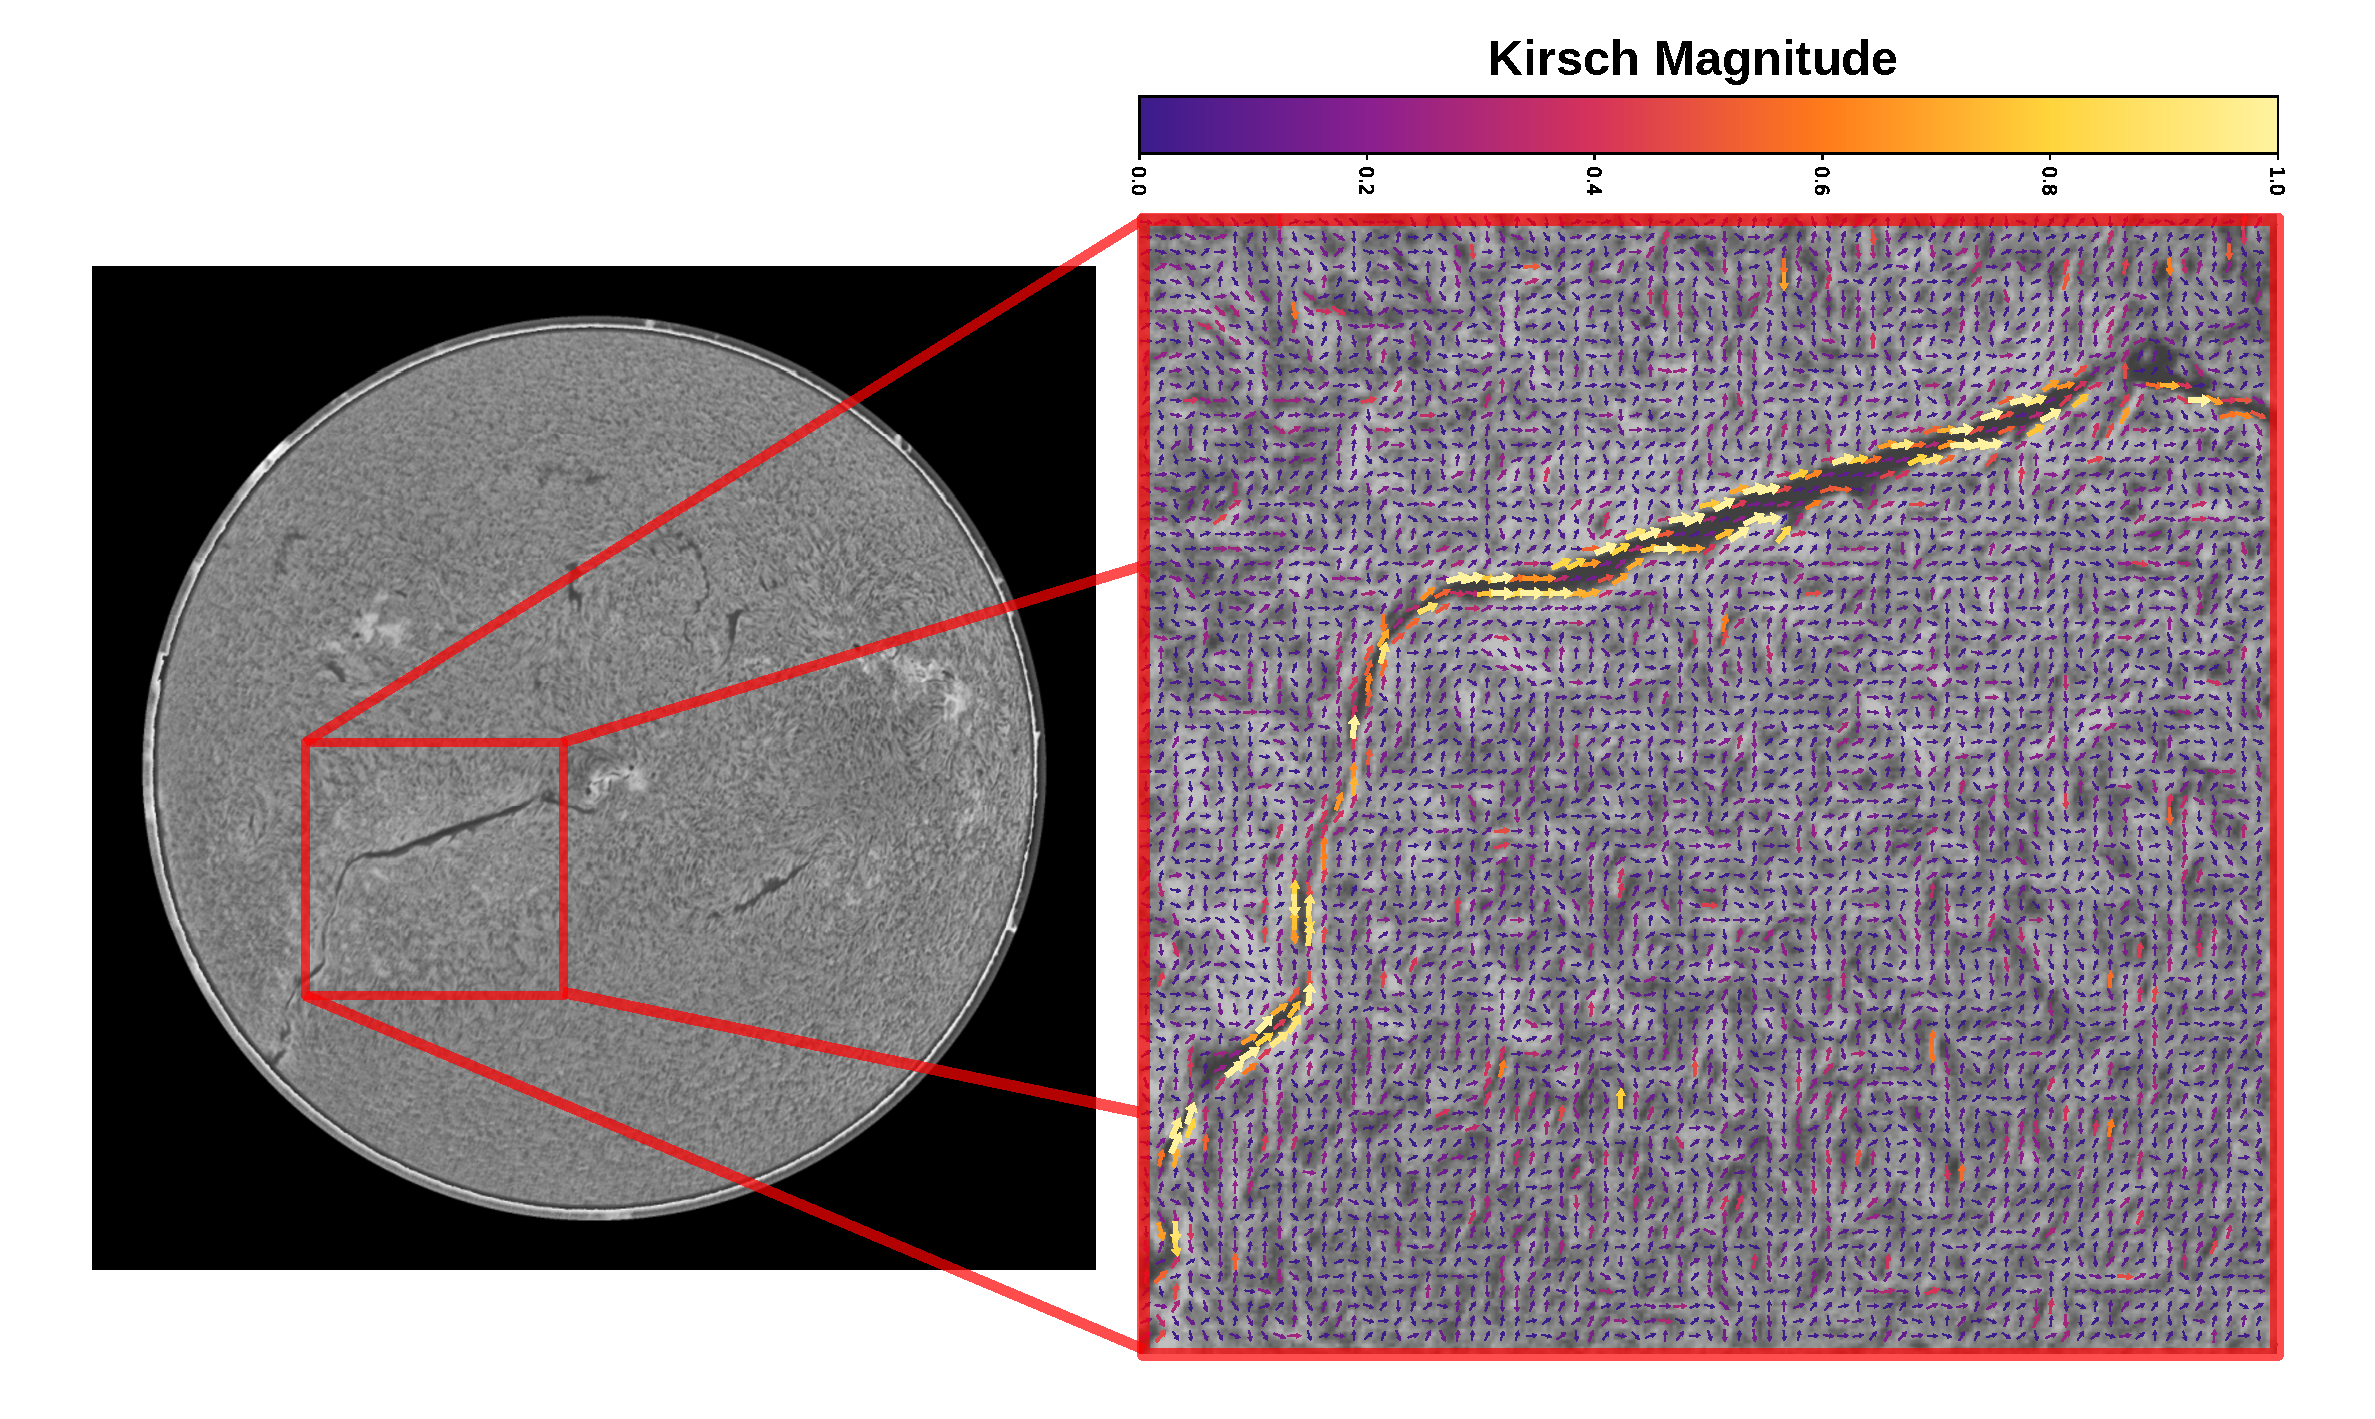
\includegraphics[width=0.75\columnwidth]{images/vector_field.pdf}
    \caption{Orientation field extracted at the first scale (dilation equals one), shown over a crop around a predicted filament. The field is block-averaged ($4\times4$) for display. Each arrow gives the local edge orientation. Arrow length and color encode the edge magnitude.}
    \label{fig:vector_field}
\end{figure} 

\subsubsection{Compass Attention}\mbox{}\

Before the bottleneck, on the output of the third ResNet stage, the Compass Attention module uses the orientation field to guide self-attention over the encoder features. First, the orientation moments are adaptively average-pooled to match the spatial resolution of the feature map. The pooled moments are then converted into normalized direction components and edge magnitude, using the same representation described in the Orientation Field Extractor. A $1 \times 1$ convolution projects this representation to the same number of channels as the encoder features. We also apply a depthwise $3 \times 3$ convolution to the features to provide positional information.

The resulting representations are added together to obtain the input to the attention block. To reduce the computational cost, we partition the feature map into non-overlapping $8 \times 8$ windows. Each window is processed independently, with its tokens passing through a pre-normalization transformer block composed of multi-head self-attention and an MLP, both with residual connections.

In addition to the standard attention logits, we compute a directional bias from the orientation moments. First, the direction components and edge magnitudes are summed across scales. The resulting direction vectors are normalized, and their magnitudes relative to the total edge response are used as confidence values. For each pair of tokens, we then add their direction vectors and normalize the result to obtain their average orientation. We compare this orientation with the relative displacement between the two tokens, also represented using a doubled angle. This gives a measure of how well the spatial displacement aligns with the local edge orientation. The alignment is multiplied by the average confidence of the two tokens, reducing the influence of regions with weak or incoherent edge responses. Finally, a learnable parameter for each attention head controls the contribution of this directional bias to the attention logits.

After attention, the windows are rearranged to recover the original spatial layout. A $1 \times 1$ convolution projects the resulting features, which are then added to the original encoder features through a residual connection. The projection is initialized with zero weights, allowing the network to initially preserve the original features and gradually learn the contribution of the attention block during training. Figure~\ref{fig:bottleneck} summarizes the Compass Attention module.

\begin{figure}[H]
    \centering
    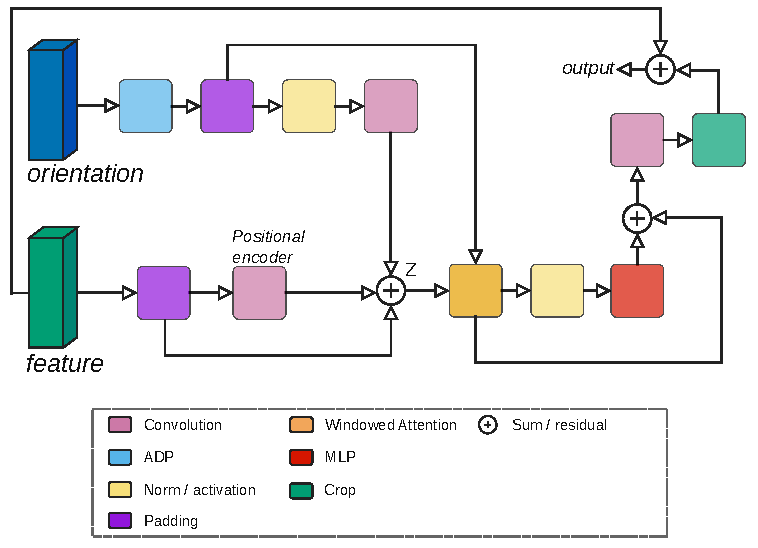
\includegraphics[width=0.75\columnwidth]{images/bottleneck.pdf}
    \caption{Compass Attention diagram.}
    \label{fig:bottleneck}
\end{figure}

\subsubsection{Orientation Conditioning}\mbox{}\

The orientation field also conditions the intermediate decoder features. At each resolution, the orientation moments are adaptively average-pooled, normalized, and projected through convolutions, Group Normalization, and GELU. The resulting features are added to the decoder representation, scaled by a learnable parameter initialized to zero, allowing the network to learn the contribution of orientation at each stage.


\subsection{Training}\label{sec:training}
\subsubsection{Self-supervised pretraining} \mbox{}\
    
    To improve our results, we pretrained the network using a self-supervised masked image completion task. The ResNet-34 encoder was initialized with ImageNet weights, and the whole network was then trained for up to 50 epochs on $5{,}000$ GONG images. The task consisted of reconstructing randomly masked image regions, with an auxiliary loss encouraging the prediction of the multi-scale orientation field extracted by the Kirsch filters. Pretraining hyperparameters, masking scheme, and losses are available in the code repository (\url{https://github.com/hermengardo/CompassNet_SolarFilamentChallenge_Solution}).
    
    We also ran a second experiment (same data) using the self-supervised method available in the LightlyTrain~\cite{lightlytrain} package. We trained the model for 300 epochs using the distillation-based module, initialized with ImageNet weights.
    
    To avoid leaking information from the supervised data into the pretraining stage, we only used GONG images acquired outside the period covered by MAGFiLO (January 9, 2011 to August 3, 2022). The $5{,}000$ pretraining images were acquired between June and September 2010 and between 2023 and 2025, across six GONG stations. The minimum gap between the self-supervised and supervised sets is 101 days before the first supervised image and 241 days after the last one.
    

\subsubsection{Supervised training} \mbox{}\
    
    Each image has several annotators. We rasterize their polygons and average them to obtain a soft mask in $[0,1]$, which is used directly as the target. By doing that, we want to encode human uncertainty into the learning process of the network. We used a hybrid loss function of BCE and Dice computed on the soft target:

    \begin{equation}
        \mathcal{L}_\text{seg} = \beta\,\mathcal{L}_\text{BCE} + (1 - \beta)\,\mathcal{L}_\text{Dice}
    \end{equation}
    
    To help the model retain structure continuity, the network also predicts the spine segmentation as an auxiliary output, supervised with the same hybrid loss ($\mathcal{L}_\text{spine}$). The total training loss is
    
    \begin{equation}
        \mathcal{L}_\text{total} = \mathcal{L}_\text{seg} + \lambda\,\mathcal{L}_\text{spine}
    \end{equation}
    
    The spine term is used only during training to guide the model. At validation time, we do not use it and report only $\mathcal{L}_\text{seg}$.

\subsubsection{Augmentations}\mbox{}\

    We mainly adopted the augmentation techniques proposed by Hu \textit{et al.} \cite{hu2026modernconvnetsolarfilament}, with the exception of random scaling, as we expected that it could destroy information about the geometry of the filaments. Table~\ref{tab:augmentation} shows the parameters.

\begin{table}[H]
    \centering
    \caption{Augmentation parameters.}
    \label{tab:augmentation}
    \footnotesize
    \renewcommand{\arraystretch}{1.12}
    \setlength{\tabcolsep}{4pt}
    \begin{tabular}{@{}llll@{}}
        \toprule
        \textbf{Augmentation} & \textbf{Probability} & \textbf{Variable} & \textbf{Range} \\
        \midrule
        Horizontal flip & 0.90 & -- & -- \\
        Vertical flip   & 0.90 & -- & -- \\
        Random rotation & 0.90 & $\theta$ & $[-45^\circ, 45^\circ]$ \\
        Random gamma    & 0.25 & $\gamma$ & $[0.5, 2.5]$ \\
        \bottomrule
    \end{tabular}
\end{table}

\subsection{Postprocessing}\label{sec:postprocessing}
    We used test-time augmentation (TTA), averaging the predicted probabilities over the eight dihedral transformations of each input. The averaged map was binarized and post-processed with an implementation adapted from Hu \textit{et al.}~\cite{hu2026modernconvnetsolarfilament}, which fills the external contours so that every region is simply connected and discards regions below a minimum area. Finally, we used Optuna (40 trials)~\cite{akiba2019optuna} to tune the minimum region area and threshold by maximizing the validation IoU (see table~\ref{tab:params}).

% ==================================== %
%              EVALUATION              %
% ==================================== %
\section{Evaluation}\label{sec:evaluation}

\subsection{Evaluation Strategy}
We report IoU (Jaccard), precision, recall, F1, and Panoptic Quality (PQ) on the validation set, using a 0.5 threshold on the sigmoid output. IoU is averaged per image, while precision, recall, and F1 are computed from pixel counts accumulated over all images.

\subsection{Benchmarks}
\subsubsection{Self-Supervised Learning}\footnote{For the benchmarks, we adopted a more conservative minimum gap of 14 days between the training and validation sets, instead of 2 days.}\mbox{}\

We trained four variants of the same CompassNet architecture with a fixed seed (6125), differing only in the initialization: random weights, an ImageNet-pretrained backbone, weights obtained by masked image completion, and weights obtained by self-supervised distillation via LightlyTrain~\cite{lightlytrain}. Uncertainty was estimated with a non-parametric bootstrap over the validation images (5{,}000 resamples with replacement). Figure~\ref{fig:results} reports point estimates with 95\% percentile confidence intervals.

\begin{figure}[H]
    \centering
    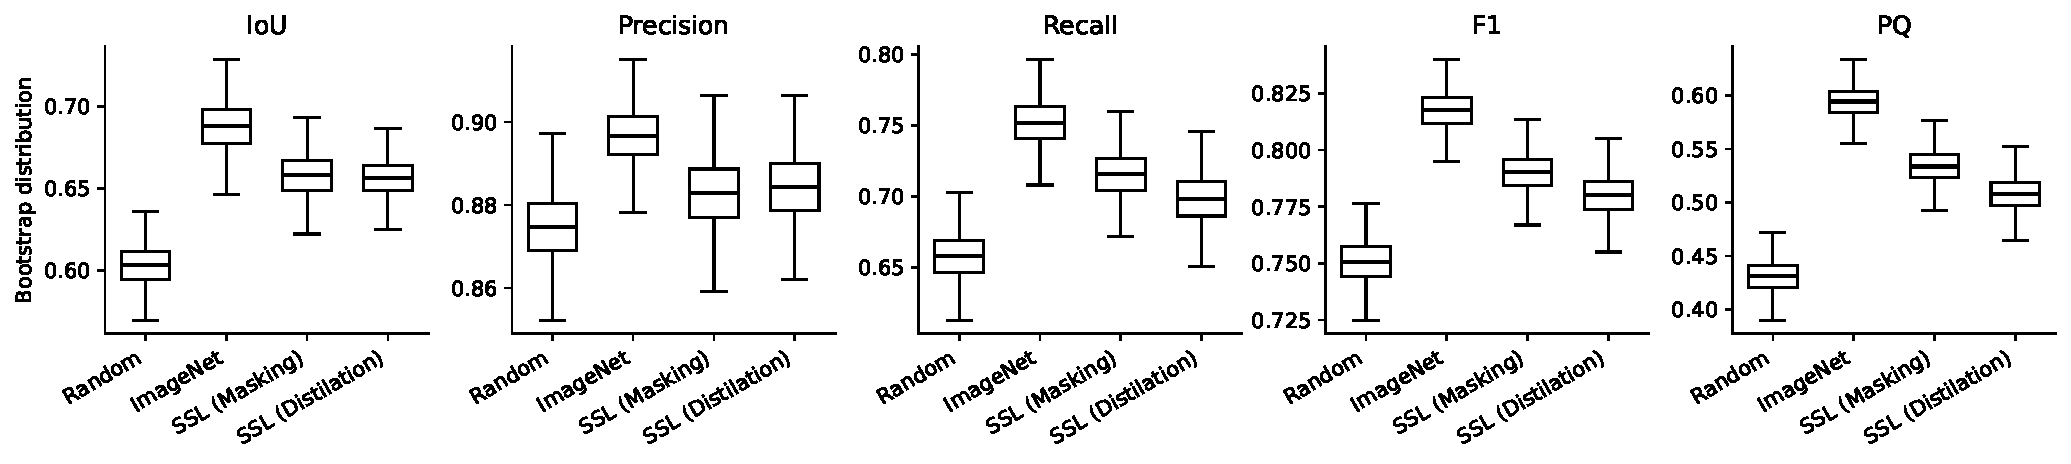
\includegraphics[width=\linewidth]{images/boxplot_backbone.pdf}
    \caption{Validation performance of backbone pretraining.}
    \label{fig:results}
\end{figure}

Both self-supervised approaches performed worse than using the standard pretrained ResNet weights directly. However, the masking-based approach achieved slightly better results than the distillation-based approach, even with fewer training epochs (50 vs. 300). Despite this, both self-supervised approaches performed better than training the model from scratch, without pretrained weights.

Figure~\ref{fig:comparison} shows qualitative comparisons between the mask generated by the final model and the corresponding ground-truth masks for a random image.

\begin{figure}[H]
    \centering
    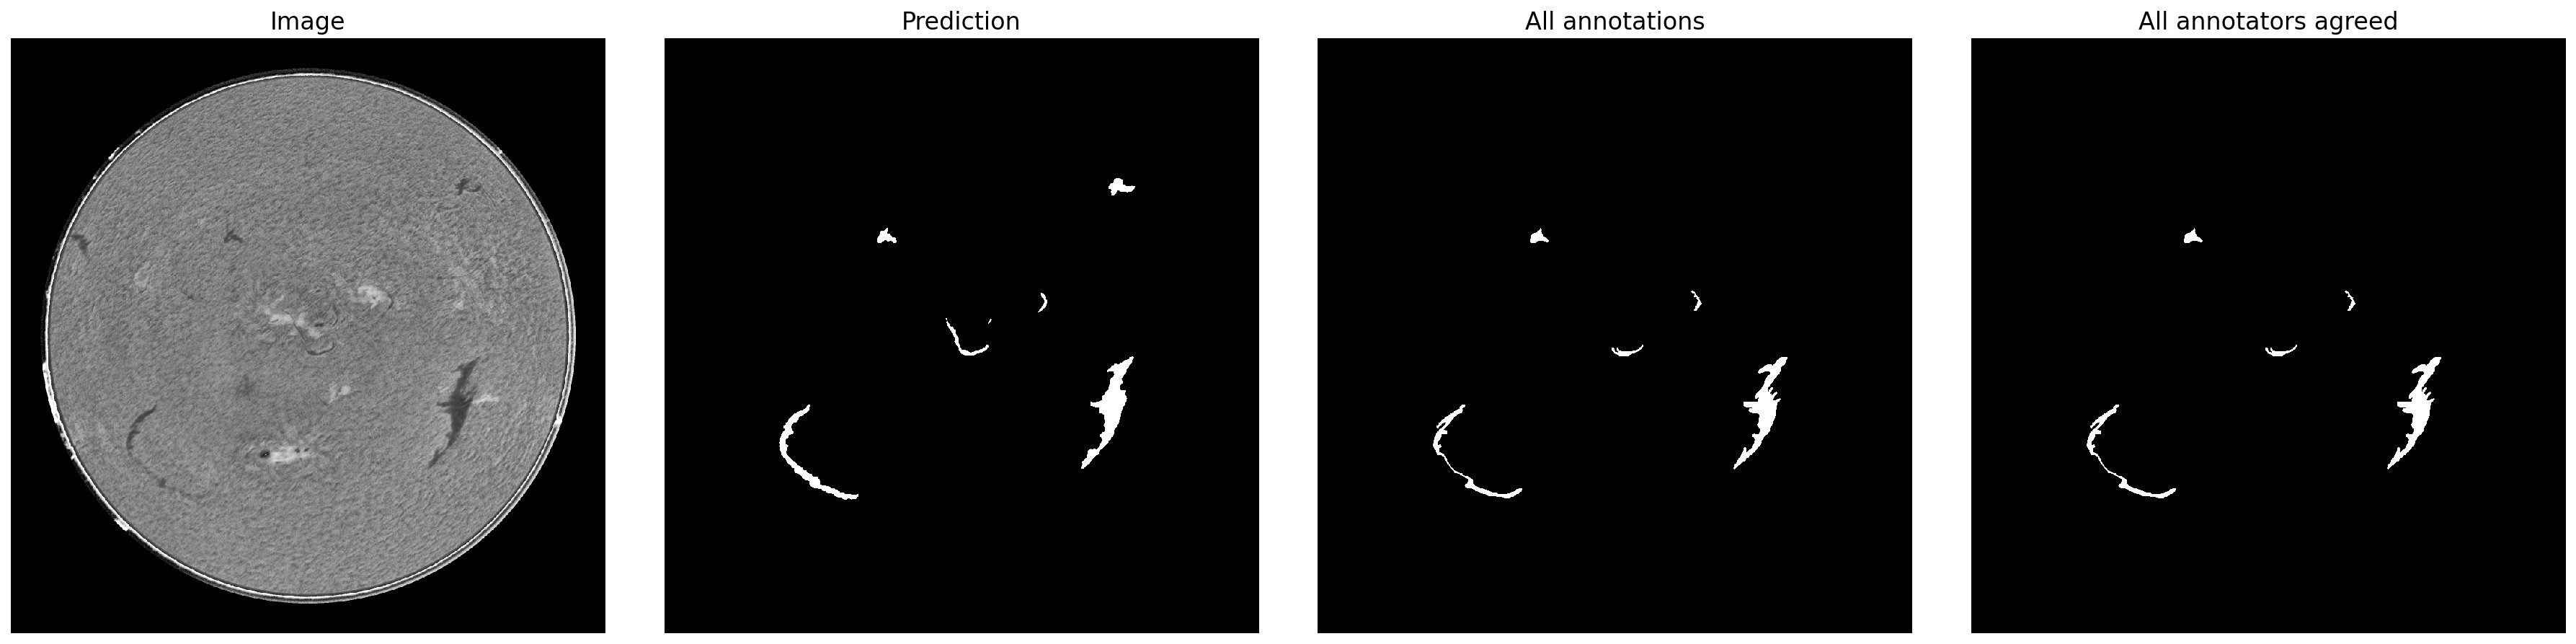
\includegraphics[width=\linewidth]{images/grid.png}
    \caption{Qualitative results on validation image. From left to right: input image, mask predicted by the model, combined annotations from all annotators, and the consensus region on which the annotators agree.}
    \label{fig:comparison}
\end{figure}

\subsubsection{Supervised Learning}\mbox{}\

For our final model, we evaluated CompassNet using the evaluation notebook provided by the competition organizers. The notebook was used to assess the model on a validation set containing 10\% of the training set size. The resulting metrics are reported in Table~\ref{tab:competition}. We did not run ablations isolating the orientation-guided components, so their individual contribution relative to a plain U-Net is not established here.

\begin{table}[H]
    \caption{Performance comparison on the validation set.}
    \label{tab:competition}
    \centering
    \small
    \begin{tabular}{lc}
        \hline
        \textbf{Metric} & \textbf{CompassNet} \\
        \hline
        Panoptic Quality (PQ) & 0.35 \\
        Mean IoU & 0.50 \\
        Mean Dice Score & 0.63 \\
        \hline
    \end{tabular}
\end{table}

\subsubsection{Final Model}\mbox{}\

We submitted a single set of predictions generated by CompassNet, without ensembling or combining predictions from other models. Table~\ref{tab:params} summarizes the model architecture, training hyper-parameters, and inference settings.
% ==================================== %
%            ACKNOWLEDGMENT            %
% ==================================== %
\section{Acknowledgment}\label{sec:acknowledgment}
    % Do not change
    The organization of the Filament Segmentation Challenge 2026 is partially supported by the U.S. National Science Foundation (NSF) under Grant No. 2209912 and 2433781, directorate for Computer and Information Science and Engineering (CSE), and Office of Advanced Cyberinfrastructure (OAC), and Grant No. 2511630, AST Division Of Astronomical Sciences and MPS Directorate for Mathematical and Physical Sciences.

    The Filament Segmentation Challenge 2026 is sponsored by the U.S. National Science Foundation (NSF) National Solar Observatory (NSO). 

    This work utilizes GONG data obtained by the NSO Integrated Synoptic Program, managed by the National Solar Observatory, which is operated by the Association of Universities for Research in Astronomy (AURA), Inc. under a cooperative agreement with the National Science Foundation and with contribution from the National Oceanic and Atmospheric Administration. The GONG network of instruments is hosted by the Big Bear Solar Observatory, High Altitude Observatory, Learmonth Solar Observatory, Udaipur Solar Observatory, Instituto de Astrofísica de Canarias, and Cerro Tololo Interamerican Observatory.

\begin{table}[H]
    \centering
    \caption{Configuration and hyperparameters of the final submitted model.}
    \label{tab:params}
    \footnotesize
    \renewcommand{\arraystretch}{1.15}
    \setlength{\tabcolsep}{5pt}
    \begin{tabular}{@{}ll@{}}
        \toprule
        \textbf{Parameter} & \textbf{Value} \\
        \midrule
        Architecture       & CompassNet \\
        Backbone           & ResNet-34 (ImageNet) \\
        Dilation rates     & (2, 4, 8) \\
        Frozen batch normalization & Yes \\
        Attention heads    & 4 \\
        $\tau$              & 0.1 \\
        \midrule
        Input resolution   & $2048 \times 2048$ \\
        Number of epochs   & 100 \\
        Batch size         & 2 \\
        Optimizer          & AdamW \\
        Learning rate      & $10^{-4}$ \\
        Weight decay       & $10^{-4}$ \\
        LR scheduler       & Cosine annealing \\
        Gradient clipping  & 1.0 (norm) \\
        Precision          & BF16 mixed precision \\
        Loss function      & $0.5\,\text{BCE} + 0.5\,\text{Dice}$ \\
        $\lambda$          & 0.05 \\
        $\beta$            & 0.5 \\
        \midrule
        Threshold          & 0.5 \\
        Minimum area       & 32 \\
        \midrule
        GPU                & NVIDIA H100 \\
        Random seed        & 567 \\
        Validation split   & 20\% \\
        \bottomrule
    \end{tabular}
\end{table}

\bibliographystyle{ACM-Reference-Format}
\bibliography{main}

\end{document}
